\section{Perancangan Sistem}
Sistem yang dikembangakan menggunakan platform Java dengan model pemrograman berorientasi objek, untuk itu pemodelan sistem menggunakan bahasa UML \emph{(Unified Modelling Language)}. Adapun diagram UML yang digunakan untuk merepresentasikan sistem adalah \emph{usecase diagram, activity diagram dan class diagram}.

\begin{figure}[th]
    \centering
    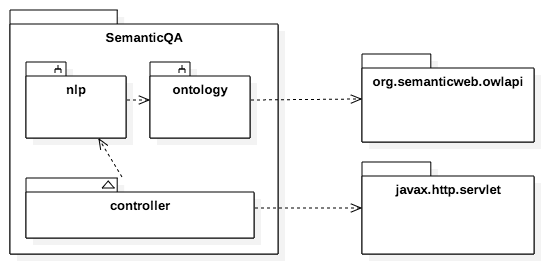
\includegraphics[width=1\textwidth]{overview_package}
    \caption{Paket sistem \emph{question answering}}
    \label{fig:overview_package}
\end{figure}

% \subsection{Diagram \emph{usecase}}
Diagram \emph{usecase} digunakan untuk menunjukkan interaksi sistem dengan aktor atau pengguna, berapa jumlah aktor serta hak akses masing-masing aktor terhadap sistem. Interaksi pengguna dengan sistem ditunjukkan dalam gambar \ref{fig:usecase_diagram} dimana sistem \emph{question answering} yang akan dibangun hanya melibatkan satu aktor yaitu pengguna yang akan memasukkan pertanyaan.

Komponen-komponen penyusun server terdiri dari tiga buah sub modul utama seperti yang ditunjukkan dalam gambar \ref{fig:overview_package}, yaitu \emph{endpoint}, nlp dan ontology. sub modul \emph{endpoint} bertindak sebagai \emph{entry point} dimana sub modul ini hanya terdiri dari satu buah kelas yaitu Main.java. Sub modul nlp berisi kelas Tokenizer, Parser dan MorphologicalAnalyzer sedangkan sub modul ontology terdiri dari dua buah kelas yaitu OntologyLoader dan OntologyQuery.

\begin{figure}[ht]
    \centering
    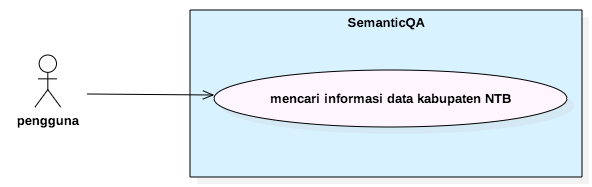
\includegraphics[width=0.8\textwidth]{usecase_diagram2}
    \caption{Diagram \emph{usecase} sistem \emph{question answering}}
    \label{fig:usecase_diagram}
\end{figure}

Selain modul utama tersebut, sistem juga menggunakan \emph{library} pihak ketiga seperti terlihata dalam gambar \ref{fig:overview_package}. Adapun \emph{library} pihak ketiga yang dibutuhkan adalah \emph{java sql connector} berfungsi sebagai konektor dengan database lexicon, \emph{jersey} sebagai library untuk membentuk web service serta \emph{owl api} untuk penanganan ontologi.

Sistem \emph{question answering} melalui beberapa tahapan pemrosesan hingga menghasilkan jawaban. Adapun tahapan-tahapan yang dilakukan oleh sistem dapat dijelaskan dengan menggunakan diagram \emph{activity} seperti ditunjukkan dalam gambar \ref{fig:activity_diagram}.

\begin{figure}[hb]
    \centering
    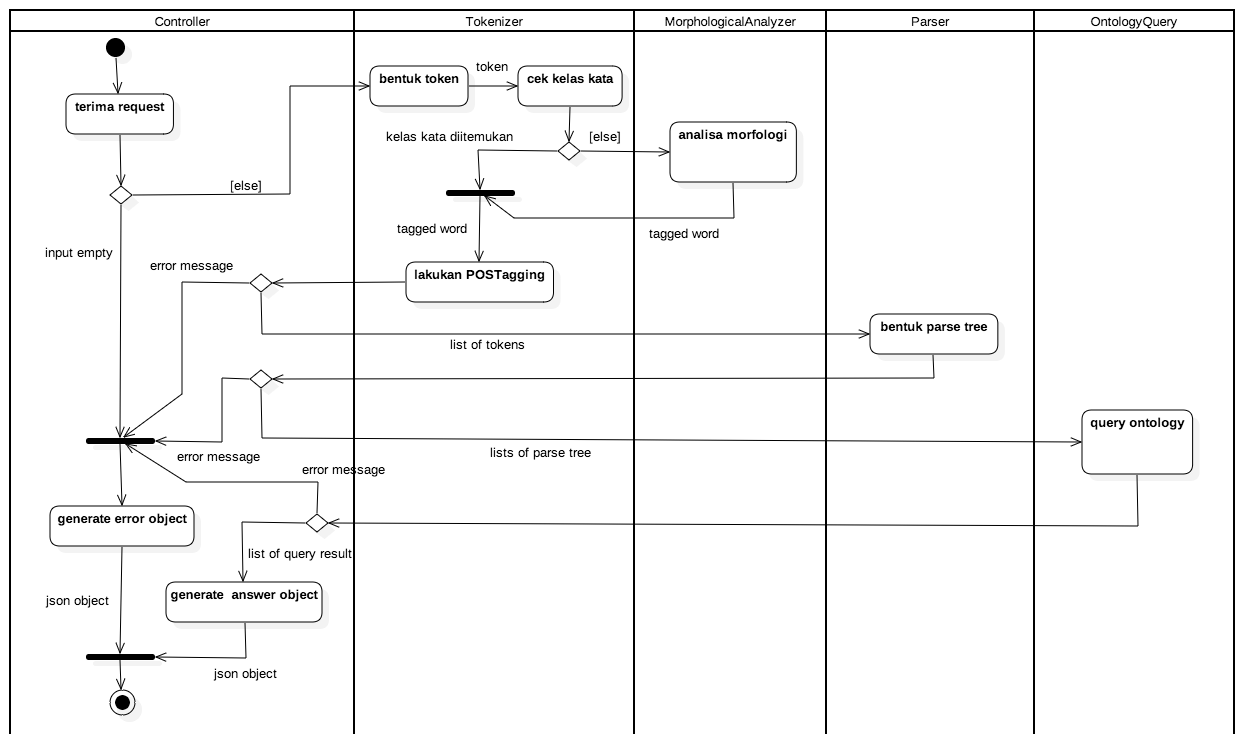
\includegraphics[width=1\textwidth]{activity_diagram}
    \caption{\emph{activity diagram}}
    \label{fig:activity_diagram}
\end{figure}

% \subsection{Diagram kelas}
% Sebelumnya telah dijelaskan bahwa sistem \emph{question answering} yang akan dikembangkan dalam penelitian ini terdiri dari beberapa modul. Masing-masing modul terdiri dari beberapa kelas dengan fungsi yang berbeda.

\subsection{Modul \emph{endpoint}}
Modul \emph{endpoint} hanya terdiri dari satu buah kelas yaitu Main.java. Kelas ini terdiri dari dua buah method yaitu \emph{search()} dan \emph{buildResponse()} seperti ditunjukkan dalam gambar \ref{fig:sub_sistem_endpoint}. Method \emph{search()} menerima masukan berupa string yang merupakan pertanyaan yang dikirimkan oleh \emph{client}, method ini memiliki akses kenampakan public.

Method \emph{buildResponse()} berfungsi untuk membentuk objek JSON yang nantinya akan dikirimkan kepada \emph{client} sebagai respon. Adapun format objek JSON yang dihasilkan adalah sebagai berikut:

\begin{lstlisting}[language=XML,xleftmargin=0pt][th]
    {
        "code" : <code>,
        "status": <pesan_teks>,
        "question": <pertanyaan>,
        "answer": <array_jawaban>
    }
\end{lstlisting}

Objek ``code'' berisi integer kode sesuai dengan kode status standar yang digunakan oleh protokol HTTP, sedangkan objek ``status'' berisi string pesan sebagai penjelasan dari objek kode. Objek ``question'' berisi kalimat pertanyaan yang dikirimakan oleh \emph{client} sedangkan ``answer'' berisi array jawaban hasil pemrosesan sistem. Array ini dapat berupa array kosong jika sistem tidak berhasil menemukan jawaban.

\begin{figure}[hb]
    \centering
    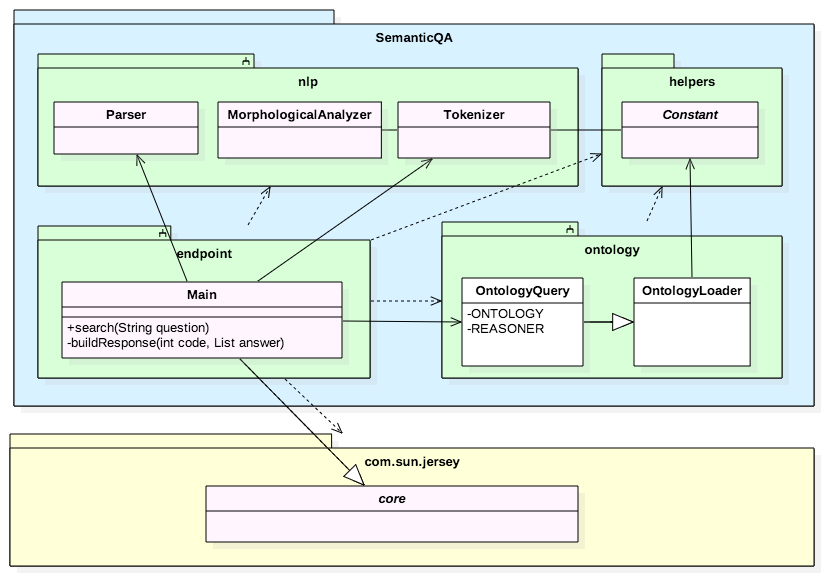
\includegraphics[width=1\textwidth]{sub_sistem_endpoint}
    \caption{Struktur dan inetraksi modul \emph{endpoint}} 
    \label{fig:sub_sistem_endpoint}
\end{figure}

Pertanyaan dikirimkan oleh \emph{client} dalam bentuk query parameter \emph{q}. Query parameter ini kemudian akan ditangkap dan diperiksa oleh method \emph{search()}. Jika query string berupa string kosong maka method \emph{search()} akan langsung memanggil method \emph{buildResponse()} dengan mengirimkan kode 204 yang mengindikasikan \emph{no content}. Jika query string dianggap valid maka method \emph{search()} akan memulai proses pencarian dengan melakukan proses tokenisasi dengan melakukan proses instansiasi kelas Tokenizer dan memanggil method \emph{tokenize()} dengan query parameter yang diterima sebelumnya sebagai parameter masukan. 

Apabila proses tokenisasi berhasil, maka selanjutnya method \emph{search()} akan melakukan instansiasi kelas Parser dan memanggil method \emph{parse()} dengan array list token sebagai masukan untuk membentuk \emph{parse tree}. Apabila proses pembentukan \emph{parse tree} gagal, dimana method \emph{parse()} tidak menghasilkan \emph{parse tree}, maka method \emph{search()} akan memanggil method \emph{generateRespone()} dengan mengirimkan kode 406 yang mengindikasikan pesan kesalahan \emph{not acceptable}.

Apabila proses pembentukan \emph{parse tree} berhasil, maka method \emph{search()} akan melakukan instansiasi kelas OntologyQuery dan akan mengirimkan \emph{array list parse tree} yang sudah dibentuk. Kembalian hasil query ontologi berupa array list yang selanjutnya akan dikirimkan ke method \emph{buildRespone()} untuk membentuk objek JSON yang selanjutnya akan dikirimkan kepada \emph{client} sebagai respon.


\subsection{Modul pemrosesan bahasa alami}
Modul pemrosesan bahasa alami terdiri dari tiga buah kelas seperti ditunjukkan dalam gambar \ref{fig:sub_sistem_nlp} yaitu: Tokenizer, MorphologicalAnalyzer dan Parser. Kelas Tokenizer berfungsi untuk merubah query string yang dikirimkan oleh \emph{client} menjadi array list token kata yang telah diberi penanda kelas kata.

\begin{figure}[ht]
    \centering
    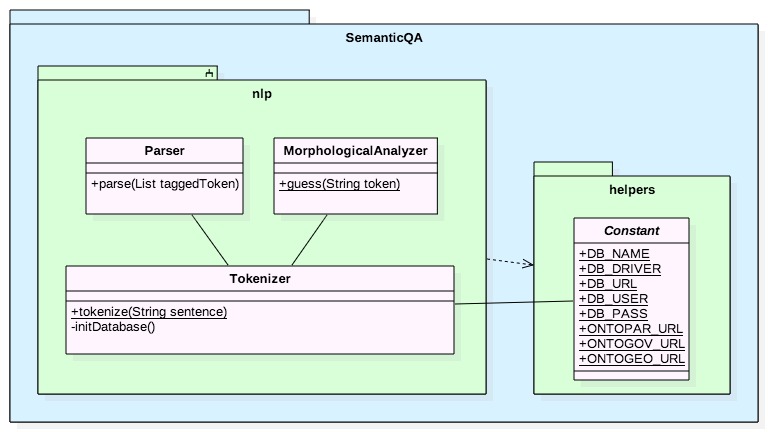
\includegraphics[width=1\textwidth]{sub_sistem_nlp}
    \caption{Struktur modul pemrosesan bahasa alami} 
    \label{fig:sub_sistem_nlp}
\end{figure}

Proses pengenalan kelas kata dilakukan dengan cara memeriksa kata yang bersangkutan ke dalam database \emph{lexicon}. Database \emph{lexicon} berupa database SQL yang berisi kumpulan kata dasar bahasa indonesia beserta dengan kelas katanya. Apabila kelas kata tidak ditemukan dalam database, maka kata yang bersangkutan dikirim ke kelas \emph{MorphologicalAnalyzer}. Method \emph{quess()} dalam kelas ini akan menebak kelas kata dengan cara melakukan analisa bentuk morfologis kata yang berangkutan berdasarkan aturan morfologi bahasa Indonesia yang dijelaskan oleh \citet{alwi}. Apabila semua aturan morfologis tidak terpenuhi, maka kata yang bersangkutan dianggap sebagai kata benda dan akan diberikan kelas kata N.

Method \emph{parse} dalam kelas Parser berfungsi untuk membentuk \emph{parse tree}. Method ini menerima masukan berupa array list kata yang telah diberi kelas kata pada proses tokenisasi sebelumnya. Pembentukan \emph{parse tree} dilakukan dengan menggunakan metode \emph{bottom-up} dimana proses pemeriksaan aturan-aturan bahasa dimulai dari konstituen kalimat yang kemudian dilanjutkan dengan frasa hingga membentuk kalimat utuh. Apabila selama proses terdapat aturan yang tidak terpenuhi, maka proses pembentukan \emph{parse tree} akan dihentikan dan pembentukan \emph{parse tree} dianggap gagal.

\subsection{Modul pemrosesan ontologi}
Struktur modul pemrosesan ontologi ditunjukan dalam gambar \ref{fig:sub_sistem_ontologi}. Modul ini merupakan modul utama yang terdri dari dua buah kelas masing-masing OntologyLoader yang berfungsi untuk memanggil ontologi dan membentuk objek java yang siap untuk di query. Pada kelas OntologyLoader juga dilakukan instansiasi objek \emph{reasoner}. Kelas OntologyQuery befungsi untuk melakukan operasi query terhadap objek ontologi yang telah dibuat dalam kelas OntologyLoader.

\begin{figure}[ht]
    \centering
    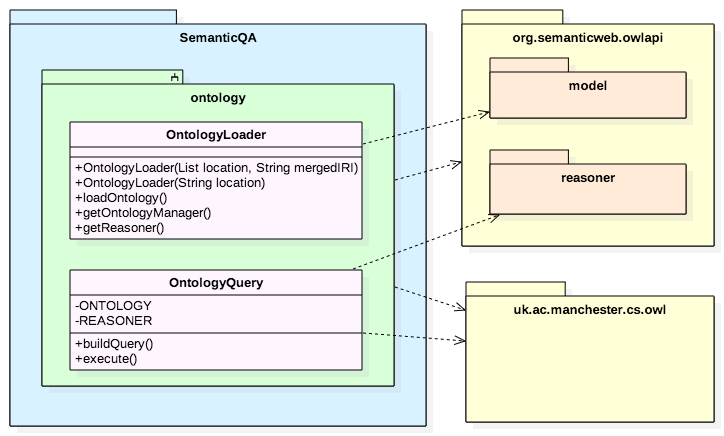
\includegraphics[width=1\textwidth]{sub_sistem_ontologi}
    \caption{Struktur modul pemrosesan ontologi} 
    \label{fig:sub_sistem_ontologi}
\end{figure}

Sebelum melakukan proses query, pertama-tama sistem akan melakukan proses pemeriksaan terhadap kelas ontologi berdasarkan \emph{parse tree} yang telah dibentuk. Pemeriksaan ini bertujuan untuk mengetahui apakah kelas yang akan dikenakan query memiliki aturan restriksi atau tidak. Jika kelas memiliki aturan restriksi, maka sistem akan memberikan tanda \emph{(flag) advanceSearch}. \emph{Flag} ini berfungsi untuk mengindikasikan bahwa selain query SPARQL nantinya juga akan dilakukan proses inferensi untuk mencari \emph{fact} yang mungkin secara implisit terdapat dalam ontologi tersebut. Hal ini dilakukan karena query SPARQL tidak dapat mencari fakta-fakta implisit yang terdapat dalam ontologi. Sebagi contoh, misalnya dalam kelas ``Bupati'', kelas ini memiliki definisi sebagai berikut:

\begin{lstlisting}[language=XML,xleftmargin=0pt]
    <EquivalentClasses>
        <Class abbreviatedIRI="dbid:Bupati"/>
        <ObjectIntersectionOf>
            <Class IRI="http://xmlns.com/foaf/0.1/Person"/>
            <ObjectSomeValuesFrom>
                <ObjectProperty abbreviatedIRI="org:headOf"/>
                <Class abbreviatedIRI="dbid:Kabupaten"/>
            </ObjectSomeValuesFrom>
        </ObjectIntersectionOf>
    </EquivalentClasses>
\end{lstlisting}

Kelas ini mungkin tidak memiliki \emph{direct instance} namun jika sebuah \emph{instance} kelas \emph{Person} memenuhi kriteria restriksi di atas maka query harus dapat menemukan \emph{instance} tersebut. Untuk itu, proses inferensi perlu dilakukan selain proses query SPARQL.



% \subsubsection{Kelas \emph{Main}}
% Kelas \emph{Main} merupakan kelas yang berfungsi sebagai \emph{controller} yang bertugas untukmengatur komunikasi antara \emph{client} dengan server. Kelas ini merupakan sub kelas dari httpServlet. Kelas \emph{Main} diletakkan dalam paket \emph{controller} sedangkan kelas httpServlet berada pada paket \emph{javax.servlet.http}

% Kelas Main terdiri dari dua buah method yaitu \emph{doGet()} dan \emph{processRequest()}. \emph{doGet()} memiliki akses kenampakan \emph{protected} dan merupakan versi \emph{overriding} dari method \emph{doGet()} pada kelas httpServlet. Method \emph{processRequest()} memiliki akses kenampakan private sehingga tidak dapat diakses dari luar atau dari web karena method ini hanya berfungsi sebagai pemroses internal yang hanya akan dipanggil melalui internal kelas Main.

% \subsubsection{Kelas Tokenizer}
% Tokenizer merupakan kelas yang berfungsi untuk melakukan proses tokenisasi terhadap kalimat tanya yang dikirimkan oleh user. Tokenizer akan menghasilkan data token berupa \emph{array list}

% \subsubsection{Kelas NGram}
% Kelas ini berfungsi untuk melakukan proses penggabungan kata per kata untuk kemudian di cek pada ontologi apakah kata yang terbentuk terdapat di dalam ontologi atau tidak. Kelas ini juga berfungsi untuk melakukan POS-Tangging terhadap token untuk menandakan tipe dari kata tersebut.

% Kelas NGram memiliki tiga buah method yaitu konstruktor, \emph{processNgram()} dan \emph{getNgram()}. method konstruktor menerima input berupa array list token sedangkan method \emph{processNgram()} tidak memiliki masukan maupun kembalian, method ini hanya digunakan untuk melakukan proses ngram secara internal, oleh karena itu kenampakannya dibuat \emph{private}. Method \emph{getNgram()} memiliki kenampakan public dengan kembalian berupa array list yang berisi string kata yang telah diberikan tag.

% \subsubsection{Kelas Ontology}
% Kelas Ontology merupakan kelas yang berfungsi untuk melakukan inisiasi ontologi. Kelas ini juga berfungsi untuk melakukan proses \emph{merging} terhadap ketiga ontologi sumber yang sudah di load sebelumnya.